\documentclass[10pt]{article}
\usepackage[margin=1in]{geometry}
\usepackage{amsmath,amssymb}
\usepackage{booktabs}
\usepackage{xcolor}
\usepackage{tikz}
\usetikzlibrary{positioning,arrows.meta,fit,calc}
\usepackage{pgfplots}
\pgfplotsset{compat=1.17}
\usepgfplotslibrary{groupplots}
\usepackage[hidelinks]{hyperref}
\usepackage{caption}
\captionsetup{font=small}
\usepackage{enumitem}
\usepackage{float}
\setlist{itemsep=2pt,topsep=3pt}

\newcommand{\Eth}{E_{\mathrm{Th}}}
\newcommand{\Emax}{E_{\max}}
\newcommand{\EL}{E_{\mathrm{L}}}

\title{DiffBHAR: training BHAR's acquisition policy with gradients\\[2pt]\large Results summary}
\author{John Xu}
\date{October 30, 2026}

\sloppy
\begin{document}
\maketitle

\section*{In one paragraph}
BHAR tunes a two-parameter send rule per sensor with pattern search on a proxy reward (active-region fraction). We make BHAR's sensor simulator differentiable and train the policy, a small per-sensor neural network, directly on the classification loss of the held prediction. Everything else is BHAR's own code: data, splits, cached TinyHAR, finetuning and test. \textbf{On 3 of 4 datasets we match BHAR's accuracy with 14--39\% fewer packets}; Opportunity (4 subjects) is worse. Giving BHAR's search 16$\times$ the budget changes neither its accuracy nor its packets. Under BHAR's harsher setting (half the harvested energy) all policies tie. The estimated on-sensor cost of the network is below the energy saved on all 4 datasets.

\section{Method}

\begin{figure}[t]
\centering
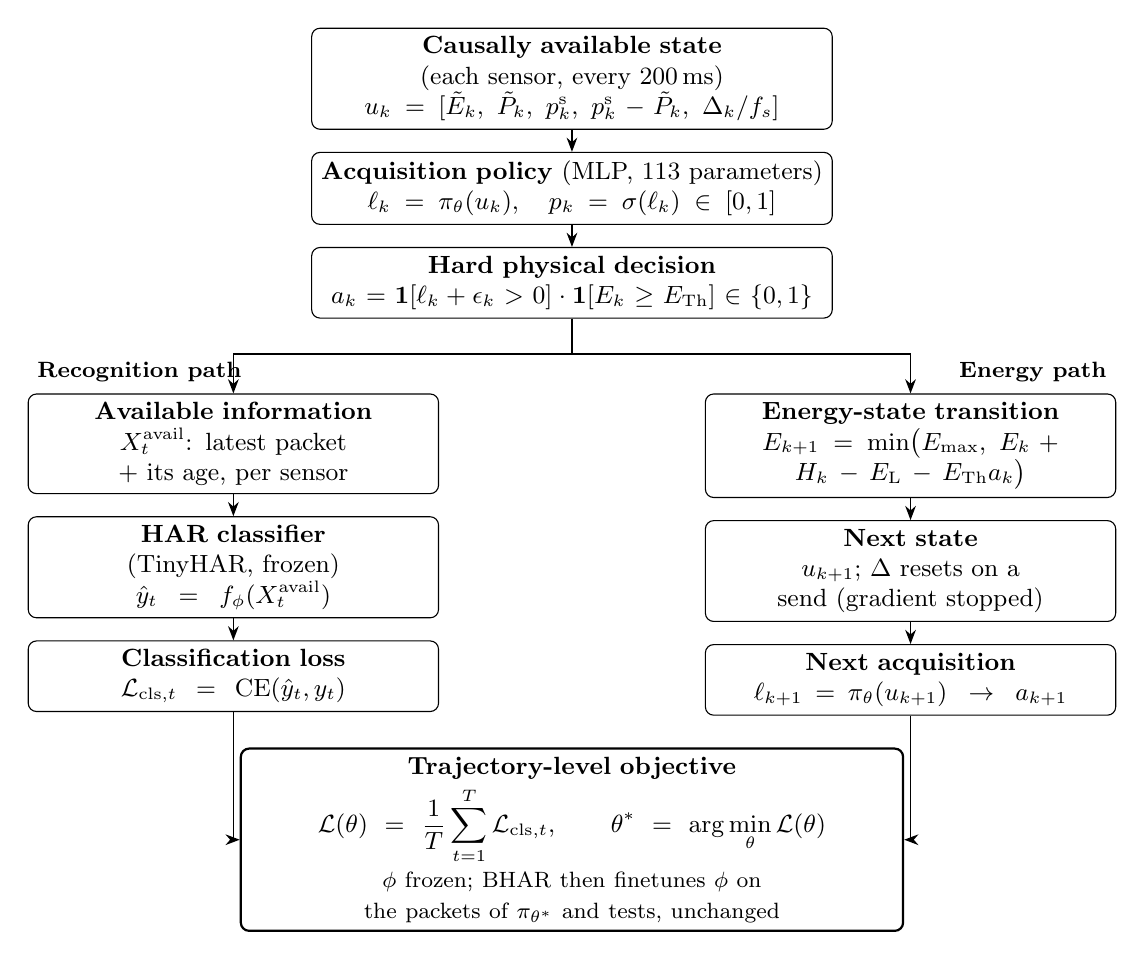
\begin{tikzpicture}[
  b/.style={draw, rounded corners=3pt, align=center, font=\small, inner sep=3pt, text width=#1},
  b/.default=6.4cm,
  a/.style={-{Stealth[length=1.8mm]}, semithick},
  lab/.style={font=\small\bfseries}]
\node[b] (s) at (0,0) {\textbf{Causally available state} (each sensor, every 200\,ms)\\
  $u_k = [\tilde E_k,\ \tilde P_k,\ p^{\mathrm s}_k,\ p^{\mathrm s}_k-\tilde P_k,\ \Delta_k/f_s]$};
\node[b, below=0.28cm of s] (p) {\textbf{Acquisition policy} (MLP, 113 parameters)\\
  $\ell_k = \pi_\theta(u_k),\quad p_k=\sigma(\ell_k)\in[0,1]$};
\node[b, below=0.28cm of p] (h) {\textbf{Hard physical decision}\\
  $a_k = \mathbf 1[\ell_k+\epsilon_k>0]\cdot\mathbf 1[E_k\ge \Eth]\in\{0,1\}$};
% left: recognition path
\node[b=5.0cm, anchor=north] (x) at ($(h.south)+(-4.3,-0.95)$) {\textbf{Available information}\\ $X^{\mathrm{avail}}_t$: latest packet + its age, per sensor};
\node[b=5.0cm, below=0.28cm of x] (c) {\textbf{HAR classifier} (TinyHAR, frozen)\\ $\hat y_t = f_\phi(X^{\mathrm{avail}}_t)$};
\node[b=5.0cm, below=0.28cm of c] (l) {\textbf{Classification loss}\\ $\mathcal L_{\mathrm{cls},t} = \mathrm{CE}(\hat y_t, y_t)$};
% right: energy path
\node[b=5.0cm, anchor=north] (e) at ($(h.south)+(4.3,-0.95)$) {\textbf{Energy-state transition}\\ $E_{k+1} = \min\!\big(\Emax,\ E_k + H_k - \EL - \Eth a_k\big)$};
\node[b=5.0cm, below=0.28cm of e] (n) {\textbf{Next state}\\ $u_{k+1}$; $\Delta$ resets on a send (gradient stopped)};
\node[b=5.0cm, below=0.28cm of n] (q) {\textbf{Next acquisition}\\ $\ell_{k+1}=\pi_\theta(u_{k+1})\ \rightarrow\ a_{k+1}$};
\node[lab, font=\footnotesize\bfseries, above=0.02cm of x.north west, anchor=south west] {Recognition path};
\node[lab, font=\footnotesize\bfseries, above=0.02cm of e.north east, anchor=south east] {Energy path};
% objective
\node[b=8.2cm, thick, anchor=north] (o) at ($(h.south |- l.south)+(0,-0.45)$) {\textbf{Trajectory-level objective}\\[2pt]
  $\displaystyle \mathcal L(\theta) = \frac1T\sum_{t=1}^{T}\mathcal L_{\mathrm{cls},t},\qquad
   \theta^* = \arg\min_\theta \mathcal L(\theta)$\\[2pt]
  {\footnotesize $\phi$ frozen; BHAR then finetunes $\phi$ on the packets of $\pi_{\theta^*}$ and tests, unchanged}};
\draw[a] (s) -- (p);
\draw[a] (p) -- (h);
\draw[a] (h.south) -- ++(0,-0.45) -| (x.north);
\draw[a] (h.south) -- ++(0,-0.45) -| (e.north);
\draw[a] (x) -- (c); \draw[a] (c) -- (l);
\draw[a] (e) -- (n); \draw[a] (n) -- (q);
\draw[a] (l.south) |- (o.west);
\draw[a] (q.south) |- (o.east);
\end{tikzpicture}
\caption{Training pipeline. Forward pass: identical to BHAR's sensor simulator (hard decisions, packet for packet). Backward pass: straight-through estimator for $a_k$ (logistic noise $\epsilon_k$), a sigmoid surrogate for the feasibility gate, $-\Eth$ for the energy a packet uses. The state uses only the capacitor voltage (stored energy $\tilde E$, harvest rate over 1\,s $\tilde P$ and 200\,ms $p^{\mathrm s}$) and the time since the last packet $\Delta$.}
\label{fig:pipeline}
\end{figure}


\paragraph{Differentiable simulator.} Forward pass identical to BHAR's \texttt{sparsify\_data} (packet for packet). Backward: straight-through estimator for the send decision, a sigmoid surrogate for the energy-feasibility gate ($E_k \ge \Eth$), and $-\Eth$ for the energy a packet uses.

\paragraph{Policy.} Every 200\,ms each sensor computes, from harvested energy only (reading the accelerometer would cost more than the sensor harvests),
\[
u_k = \big[\tilde E_k,\ \tilde P_k,\ p^{\text{short}}_k,\ p^{\text{short}}_k-\tilde P_k,\ \Delta_k/f_s\big]:
\]
stored energy, harvest rate over 1\,s and over 200\,ms (a free proxy for motion, since harvesting is kinetic), their difference, and time since the last packet. A per-sensor MLP gives the send logit, $\ell_k = w_2^\top \tanh(W_1 u_k + c_1) + c_2$ with 16 hidden units: 113 parameters, $\sim$100 multiply--adds per decision. BHAR's rule, send if $\Delta_k \ge \theta_e(1-\tilde E_k)\tilde P_k + \theta_p$, uses a subset of these inputs.

\paragraph{Loss.} Cross-entropy of the held prediction at every time step, i.e.\ the total (active + passive) error that BHAR's reward approximates. The classifier is frozen during policy training.

\paragraph{Exploding gradient (found and fixed).} When the rule binds, each packet's time depends on the previous one through the reset of $\Delta$; the backward pass multiplies by $\approx 0.05(\Delta + 9)$ per packet, about 10 at $\theta_p=200$, so gradients reached $10^{10}$--$10^{20}$ with random sign. Stopping the gradient through the reset (forward unchanged) gives correct gradient directions ($t = 2$--$8$ on real data).

\paragraph{Training} (per test subject and seed, BHAR's training/validation sequences):
(1) the network imitates the fixed rule $\theta = (0,100)$ (chosen once on PAMAP2, never re-tuned);
(2) 16 epochs $\times$ 64 random 100\,s segments, Adam;
(3) keep the policy with the lowest validation loss (the start included);
(4) BHAR's finetuning and test, unchanged.

\section{Results}
Leave-one-subject-out, 3 seeds, BHAR's protocol (same-subject validation split). BHAR is our rerun of BHAR's code (within seed noise of the authors' cached numbers; opportunistic matches exactly).

\begin{table}[H]
\centering
\caption{Test accuracy / F1 / packets per second per sensor. Fixed (0,100) is our starting rule without training.}
\label{tab:main}
\resizebox{\textwidth}{!}{%
\begin{tabular}{lcccc}
\toprule
 & PAMAP2 & DSADS & RWHAR & Opportunity \\
\midrule
Opportunistic & .510 / .454 / .261 & .547 / .526 / .257 & .614 / .636 / .332 & .575 / .537 / .139 \\
BHAR & .573$\pm$.004 / .522 / .196 & .575$\pm$.007 / .564 / .178 & .638$\pm$.013 / .653 / .255 & .581$\pm$.023 / .544 / .123 \\
Fixed (0,100), no training & .574$\pm$.005 / .532 / .137 & .577$\pm$.016 / .566 / .147 & .625$\pm$.012 / .638 / .145 & .574$\pm$.007 / .560 / .108 \\
\textbf{Ours} & \textbf{.578}$\pm$.005 / \textbf{.531} / \textbf{.144} & \textbf{.586}$\pm$.012 / \textbf{.574} / \textbf{.153} & .635$\pm$.016 / .647 / \textbf{.155} & .555$\pm$.020 / .541 / \textbf{.111} \\
\midrule
Ours vs.\ BHAR (acc / packets) & $+0.5$ / $-27\%$ & $+1.1$ / $-14\%$ & $-0.3$ / $-39\%$ & $-2.6$ / $-9\%$ \\
\bottomrule
\end{tabular}}
\end{table}

\begin{figure}[H]
\centering
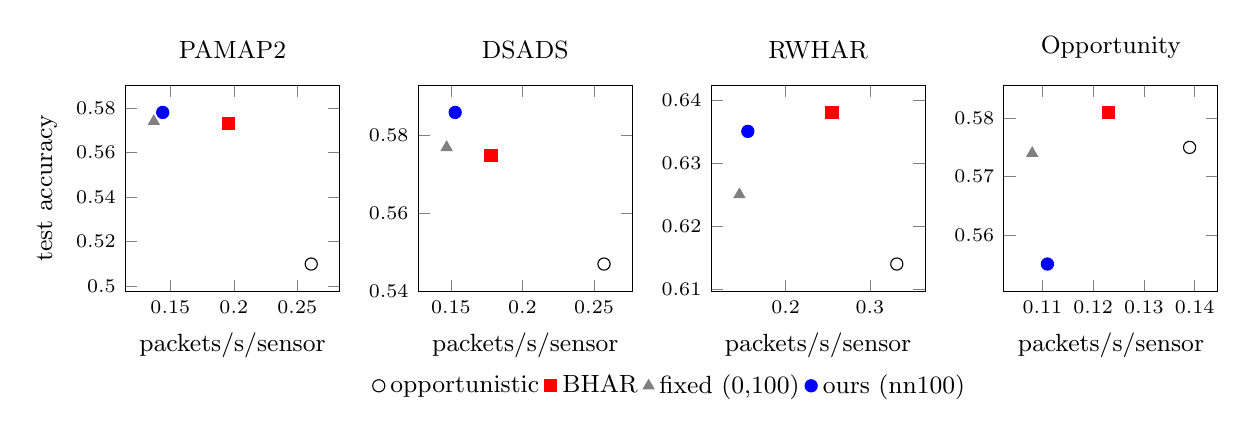
\begin{tikzpicture}
\begin{groupplot}[group style={group size=4 by 1, horizontal sep=1.0cm},
  width=4.3cm, height=4.2cm, xlabel={packets/s/sensor}, ylabel style={font=\small}, xlabel style={font=\small},
  tick label style={font=\scriptsize}, title style={font=\small}, every axis plot/.append style={only marks, mark size=2.2pt}, enlargelimits=0.18]
\nextgroupplot[title=PAMAP2, ylabel={test accuracy}]
\addplot[mark=o, black] coordinates {(0.261,0.510)};
\addplot[mark=square*, red] coordinates {(0.196,0.573)};
\addplot[mark=triangle*, gray] coordinates {(0.137,0.574)};
\addplot[mark=*, blue] coordinates {(0.144,0.578)};
\nextgroupplot[title=DSADS]
\addplot[mark=o, black] coordinates {(0.257,0.547)};
\addplot[mark=square*, red] coordinates {(0.178,0.575)};
\addplot[mark=triangle*, gray] coordinates {(0.147,0.577)};
\addplot[mark=*, blue] coordinates {(0.153,0.586)};
\nextgroupplot[title=RWHAR]
\addplot[mark=o, black] coordinates {(0.332,0.614)};
\addplot[mark=square*, red] coordinates {(0.255,0.638)};
\addplot[mark=triangle*, gray] coordinates {(0.145,0.625)};
\addplot[mark=*, blue] coordinates {(0.155,0.635)};
\nextgroupplot[title=Opportunity, legend to name=paretoleg, legend columns=4, legend style={font=\small, draw=none}]
\addplot[mark=o, black] coordinates {(0.139,0.575)}; \addlegendentry{opportunistic}
\addplot[mark=square*, red] coordinates {(0.123,0.581)}; \addlegendentry{BHAR}
\addplot[mark=triangle*, gray] coordinates {(0.108,0.574)}; \addlegendentry{fixed (0,100)}
\addplot[mark=*, blue] coordinates {(0.111,0.555)}; \addlegendentry{ours (nn100)}
\end{groupplot}
\node at ($(group c2r1.south)!0.5!(group c3r1.south)+(0,-1.2)$) {\pgfplotslegendfromname{paretoleg}};
\end{tikzpicture}
\caption{Accuracy vs.\ packets (up and left is better). Our policy sits left of BHAR at equal or higher accuracy on PAMAP2, DSADS and RWHAR.}
\label{fig:pareto}
\end{figure}


\paragraph{Training itself helps.} Over the untrained start: PAMAP2 $+0.4$, DSADS $+0.9$ (all 8 subjects improve), RWHAR $+1.0$ (8 of 11). The start rule carried over from PAMAP2 is below BHAR on RWHAR and Opportunity; training brings it to BHAR's level or above on 3 of 4 datasets without per-dataset tuning.

\paragraph{Not a compute advantage.} BHAR's search sees 62 segments per sensor, ours 1024. With 512 search epochs (1024 segments) BHAR gets .574 / .525 / .200 packets on PAMAP2, unchanged from .573 / .522 / .196.

\paragraph{Scarcer energy (BHAR's sensitivity setting).} Harvesting efficiency 0.5$\to$0.25 on PAMAP2 (BHAR's Fig.~11d), everything else unchanged; BHAR re-searched, our recipe and start rule not re-tuned. Accuracy / F1 / packets: BHAR .446 / .413 / .094, fixed (0,100) .447 / .410 / .099, ours .449 / .413 / .101 (3 seeds). All three tie and are close to opportunistic (.110 packets): with half the energy almost every affordable packet has to be sent, so no policy has room to choose, and our packet saving disappears. The gain of a learned policy is limited to moderate energy budgets.

\paragraph{Deployment cost (estimate).} The policy's inputs come from the capacitor-voltage readings BHAR already takes, so no extra sensing. We compiled one decision of the 16-unit MLP for the nRF52832 (Cortex-M4F, 64\,MHz; \texttt{gcc -O3}) and counted cycles; at 3.7\,mA and 3\,V (datasheet, running from flash) a cycle costs $\approx$0.17\,nJ. Float with a rational $\tanh$: about 1{,}000 cycles, \textbf{0.17\,$\mu$J per decision}; 8-bit weights with a $\tanh$ lookup table: about 530 cycles, \textbf{0.09\,$\mu$J}; weights take 452\,B (float) or 113\,B (8-bit). BHAR's rule is 10 instructions (negligible). For comparison, Learned Sampling (BSN 2025) measures 0.2\,$\mu$J per policy evaluation on the same MCU.

The network only matters when a packet is affordable ($E_k \ge \Eth$); otherwise the sensor compares the voltage with the threshold, as BHAR does, and skips it. Replaying our policies on the test data, this is the case at 50\% (PAMAP2), 51\% (DSADS), 58\% (RWHAR) and 31\% (Opportunity) of the 200\,ms steps. Against the packets saved ($\Eth = 50$\,$\mu$J), in $\mu$W per sensor:

\begin{center}\small
\begin{tabular}{lcccc}
\toprule
 & PAMAP2 & DSADS & RWHAR & Opportunity \\
\midrule
Packets saved vs.\ BHAR (/s/sensor) & .052 & .024 & .101 & .012 \\
Energy saved & 2.62 & 1.21 & 5.04 & 0.58 \\
Network runs (fraction of steps) & 50\% & 51\% & 58\% & 31\% \\
Policy cost, float, every step & 0.90 & 0.90 & 0.90 & 0.90 \\
Policy cost, float, only if $E_k \ge \Eth$ & 0.45 & 0.45 & 0.52 & 0.27 \\
Policy cost, 8-bit, only if $E_k \ge \Eth$ & 0.22 & 0.23 & 0.26 & 0.14 \\
\midrule
\textbf{Net}, float, every step & +1.72 & +0.31 & +4.14 & $-$0.32 \\
\textbf{Net}, 8-bit, only if $E_k \ge \Eth$ & \textbf{+2.40} & \textbf{+0.98} & \textbf{+4.78} & \textbf{+0.44} \\
\bottomrule
\end{tabular}
\end{center}

Cycle counts are estimates from the compiled code, not measurements, and the policy cost is not in the simulator (the gated 8-bit version would lower the harvest rate by about 0.2\,$\mu$W, against $\EL = 6.6$\,$\mu$W). Whether 8-bit weights change any decision is still to be checked. Total sensor power (6.6\,$\mu$W idle + packets + policy) is 10\% (PAMAP2), 2\% (DSADS), 21\% (RWHAR) lower than BHAR's and 2\% higher on Opportunity with the ungated float policy; the main gain is fewer radio transmissions at equal accuracy.

\paragraph{Limitation: Opportunity.} Only 3 training subjects per fold; training makes 3 of 4 test subjects worse (worse timing, same coverage), i.e.\ it overfits the training subjects. Two regularisers (more orderings of the training data; a KL penalty towards the start) did not fix it. BHAR is only 0.6 points above opportunistic there, within its own seed spread.

\paragraph{Side findings.} (i) Simple fixed rules dominate BHAR on PAMAP2: $\theta=(0,100)$ has the same accuracy with 30\% fewer packets. (ii) BHAR's same-subject validation split favours subject-sensitive policies (it cannot see rules that collapse to opportunistic on a new subject), which limits what any policy optimiser can gain under this protocol.

\section{Questions}
\begin{enumerate}
\item Is this worth a paper as it stands (equal accuracy, 14--39\% fewer packets, no gain under scarce energy)?
\item Venue: a 4-page letter now (IEEE Embedded Systems Letters), or DAC (Nov 18) / CODES (late March) first with these results?
\item How should Opportunity be handled, and is its spread (BHAR $\pm$.023, cache .598 vs.\ our rerun .581) known?
\end{enumerate}

\end{document}
